\documentclass[letterpaper,12pt]{article}

\usepackage{fontspec,xltxtra,xunicode}      %可使用系统自带字体
%\usepackage{}

\usepackage{setspace}    %使用行间距宏包
\usepackage{geometry}
\usepackage{graphicx}
\usepackage{amssymb}
\usepackage{indentfirst}
\usepackage{enumerate}
\usepackage{amsmath}
\usepackage{abstract}
\usepackage[slantfont, boldfont]{xeCJK}
\usepackage[colorlinks,linkcolor=black,anchorcolor=black,citecolor=black]{hyperref}
\usepackage{titlesec}
\usepackage{latexsym}
\usepackage{amsbsy}
\usepackage{amsthm}
\usepackage{amsfonts}
\usepackage{tocvsec2}
\usepackage{longtable}
\usepackage{booktabs}                % 用于表格中加下划线
\usepackage{fancyhdr}                % 页眉页脚
\usepackage{makeidx}                 % 建立索引
\usepackage{bbding}                  % 一些特殊符号
\usepackage{cite}                    % 支持引用
\usepackage{multirow}                %使用多栏宏包
\setlength{\skip\footins}{0.5cm}     % 脚注与正文的距离

\usepackage{listings}
\usepackage{xcolor}



\newcommand{\upcite}[1]{\textsuperscript{\textsuperscript{\cite{#1}}}}  %设置上标引用
\geometry{top=1.2in,bottom=1.2in,left=1.2in,right=1in}  %设置页边距
\defaultfontfeatures{Mapping=tex-text}
\XeTeXlinebreaklocale "zh"
\XeTeXlinebreakskip = 0pt plus 1pt minus 0.1pt   %设置文章内自动换行
%\setlength{\parindent}{2em}  %设定首行缩进


%英文字体设置
\setmainfont{Times New Roman}
\setsansfont{Arial}
\setmonofont{Consolas}

%设置字体大小
\newcommand{\chuhao}{\fontsize{42pt}{\baselineskip}\selectfont}      %初号字体
\newcommand{\xiaochu}{\fontsize{36pt}{\baselineskip}\selectfont}  %小初号字体
\newcommand{\yihao}{\fontsize{28pt}{\baselineskip}\selectfont}       %一号字体
\newcommand{\erhao}{\fontsize{21pt}{\baselineskip}\selectfont}       %二号字体
\newcommand{\xiaoer}{\fontsize{18pt}{\baselineskip}\selectfont}   %小二号字体
\newcommand{\sanhao}{\fontsize{15.75pt}{\baselineskip}\selectfont}   %三号字体
\newcommand{\sihao}{\fontsize{14pt}{\baselineskip}\selectfont}       %四号字体
\newcommand{\xiaosi}{\fontsize{12pt}{\baselineskip}\selectfont}   %小四号字体
\newcommand{\wuhao}{\fontsize{10.5pt}{\baselineskip}\selectfont}     %五号字体
\newcommand{\xiaowu}{\fontsize{9pt}{\baselineskip}\selectfont}    %小五号字体
\newcommand{\liuhao}{\fontsize{7.875pt}{\baselineskip}\selectfont}   %六号字体
\newcommand{\qihao}{\fontsize{5.25pt}{\baselineskip}\selectfont}     %七号字体

%更新目录指令
\renewcommand{\contentsname}{ \centerline {\heiti \sanhao{目\quad 录}}}
\renewcommand{\refname}{\centerline {\heiti \xiaosi{参考文献}}}


%listing set for Matlab code
%\lstset{ %  
%extendedchars=false,            % Shutdown no-ASCII compatible  
%language=Matlab,                % choose the language of the code  
%basicstyle=\footnotesize\tt,    % the size of the fonts that are used for the code  
%tabsize=3,                            % sets default tabsize to 3 spaces  
%numbers=left,                   % where to put the line-numbers  
%numberstyle=\tiny,              % the size of the fonts that are used for the line-numbers  
%stepnumber=1,                   % the step between two line-numbers. If it's 1 each line  
%                                % will be numbered  
%numbersep=5pt,                  % how far the line-numbers are from the code   %  
%keywordstyle=\color[rgb]{0,0,1},                % keywords  
%commentstyle=\color[rgb]{0.133,0.545,0.133},    % comments  
%stringstyle=\color[rgb]{0.627,0.126,0.941},      % strings  
%backgroundcolor=\color{white}, % choose the background color. You must add \usepackage{color}  
%showspaces=false,               % show spaces adding particular underscores  
%showstringspaces=false,         % underline spaces within strings  
%showtabs=false,                 % show tabs within strings adding particular underscores  
%frame=single,                 % adds a frame around the code  
%captionpos=b,                   % sets the caption-position to bottom  
%breaklines=true,                % sets automatic line breaking  
%breakatwhitespace=false,        % sets if automatic breaks should only happen at whitespace  
%title=\lstname,                 % show the filename of files included with \lstinputlisting;  
%                                % also try caption instead of title  
%mathescape=true,escapechar=?    % escape to latex with ?..?  
%escapeinside={\%*}{*)},         % if you want to add a comment within your code  
%%columns=fixed,                  % nice spacing  
%%morestring=[m]',                % strings  
%%morekeywords={%,...},%          % if you want to add more keywords to the set  
%%    break,case,catch,continue,elseif,else,end,for,function,global,%  
%%    if,otherwise,persistent,return,switch,try,while,...},%  
%}  

% listing set for R output
\lstset{
basicstyle=\scriptsize\tt,
}




\title{STT 864 \quad Final Project Report}
\author{Peide Li}
\date{}

\begin{document}
\maketitle

\renewcommand{\abstractname}{Summary}

\begin{abstract}
The city Flint in Michigan State has been disturbing by a water crisis for two years. The ageing pipes of the water supply system cause a high level of lead and copper in the water, which are harmful to people's health. According to the sample surveys recently, the contamination situation have become better and the water in most part does not contain lead or copper. However, the contamination still exists. In this report, I use a statistical model to explore the whether, in a certain site, a extremely high level of lead contamination (greater than 15 PPB.) would happen. I find out that, using lead pipes for home water supply system would possibly increase the probability that a high level contamination situation would happen. And in the area of Flint city, the water in where zip code are 48505 and 48507 many not be strongly affected by the contamination. Thus the water in these region is probably safe for daily use.
\end{abstract}
%%%%%%%%%%%%%%%%%%%%%%%%%%%%%%%%%%%%%%%%%%%%%%%%%%%%%%%%%%%%%%%%%%%%%%%%%%%%%%%%%%%%%%%%%%%%%%%%%%%%%%%%%%%%%%%%%%%%%%%%%%%%%%%%%%

\section*{\sihao Problem Description}
Started in April 2014, a water crisis has been disturbing Flint, a city of Michigan, for about 2 years. After the city changed its water source from treated Detroit Water and Sewerage Department water to the Flint River, its drinking water had a series of problems that culminated with lead contamination, creating a serious public health danger. According to the researches from the government, the ageing pipes, which may contain high percentage of lead, copper and other metal, are the guilty of this water crisis. The lead in the pipes leached into the water supply and causing a high lead level in the water supply system. As a result, thousands of people have been exposed to drinking water with high levels of mental elements such as lead, and they may experience a range of serious health problems. Till the end of 2015, the percentage of the incidence that elevated blood lead larger than $5mcg/dl$ among children younger than 6 in Flint city is still the highest in the Michigan State.  

In order to find a way that may be able to explain how the lead level in the Flint change, I decide to build a statistic model with the data provided by the government of Flint city. The data which would be used to fit the model, is consists of four rounds surveys about the lead concentration in the water supply system of Flint city, which can be found on Flint water website.
%\begin{center}
%\begin{figure}[ht]
%\quad  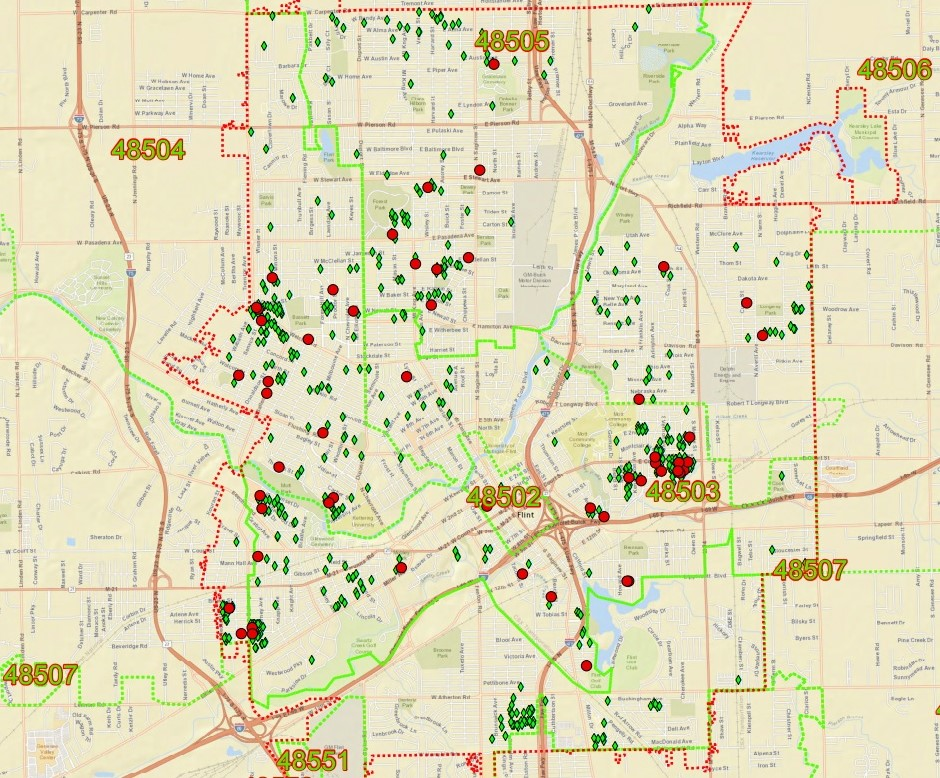
\includegraphics[width = 14cm, height = 10cm]{Sentinel_location.jpg}
%\vfill
%\caption{Sentinel Location Distribution}
%\label{fig:res}
%\end{figure}
%\end{center}

%%%%%%%%%%%%%%%%%%%%%%%%%%%%%%%%%%%%%%%%%%%%%%%%%%%%%%%%%%%%%%%%%%%%%%%%%%%%%%%%%%%%%%%%%%%%%%%%%%%%%%%%%%%%%%%%%%%%%%%%%%%%%%%%%%%%%%%
\section*{\sihao Data Processing}
The attributes in the data set are sample dates, lead and copper level, address and zip code of the site, service line material and the sample location. Since the background researches pointed out that the lead contamination is largely due to the corruption of the ageing pipes, I am interested about how the material of pipes would influence the lead and copper level in the water supply system. Besides, I think the location of the sites would be very important because people want to know the difference of lead level in the water in different areas. If we can specify where the lead level is extremely high, then governors can apply more resources to that area so that the limited resources can be fully used. And for the three attributes in the data set which all denote for the locations, I choose zip code to be the variables in my model. This is because the number of levels for zip code is not so large and can be representative at the meanwhile. So the predictor for my model would be service line material and zip code. 

As for the rest of the attributes, I do not think they would be helpful in interpreting the response variables. Sample locations, like taking samples in the bathroom or in the kitchen, are not very interesting to explore. Because for most sites, the water in the kitchen and in the bathroom would come from the same water supply systems. So the difference between them would not so significant. And, even if we can find the difference between them, the suggestion like only using the water in your kitchen would be difficult for practice. However, there is no evidence to show that the sample location would not have any effect to the lead level in the water. So, I assume sample locations to be random effects in my model. I do not include the sample dates as a factor here. It is because I want the model can be used to predict new response values. If sample dates are included, there would be a total new level of sample date when I apply the model to do prediction. So here, I assume sample dates do not influence the response variables.

\noindent Then, I refined the data set with following rules:
\begin{itemize}
\item Select the data from the zip code 48503 ~ 48507, which represent the majority of the Flint city area.
\item Select the data whose service line material are lead, copper and galvanized material. These three types of pipe are widely used in the city.
\item Select the data whose sample locations are kitchen, basement and bathroom, which are the most common in the data set.
\end{itemize}

%%%%%%%%%%%%%%%%%%%%%%%%%%%%%%%%%%%%%%%%%%%%%%%%%%%%%%%%%%%%%%%%%%%%%%%%%%%%%%%%%%%%%%%%%%%%%%%%%%%
\section*{\sihao Model Selection}
When I consider models, there are two things that I want to predict with the help of the model. One is the lead level, and the other is whether the lead level would be greater than 15 PPB. in the water system. The United States Environmental Protection Agency pointed out that if the lead level in the drinking water is greater than 15 PPB, then they would take actions to prevent the possible diseases caused by the water. In the former case, the response variable in my data set, lead values, can be transformed to a binary form. 1 denotes that the lead level in the data set is greater than 15 PPB while 0 denotes the lead level is less than 15. In this way, I can also use a logistic regression model to fit my data set.

Apart from the two choices of response variables, the model should also can include random effects, because the sample location is a random effect for the lead level. As a result, linear mixed effect model and generalized linear mixed effect model are two possible candidates. Both of them can include random effects, but linear model can predict the actually value of lead in the water, and generalized linear mixed model can predict the probability whether the lead level in the water supply system would be greater 15 PPB or not.

Since the generalized linear mixed model and linear mixed model are both meaningful under the situation, I decided to go through the data set and try to find out which model is more appropriate when I only have such a data set. Then I begin to think about the possible distribution of the lead levels. This is because for linear mixed effect model, the random error should be normally distributed. If a linear model can be appropriately applied here, then the lead value in each situations should also have a normal distribution. If the lead level is not normally distributed, then a linear model would not give out a good fit here. So for next step, I want to check the empirical distribution of the lead level data and then decide whether a linear model would be useful here.


\section*{\sihao Model for Lead Level}

The figure 1 shows the distribution plots of lead levels in different situations. The lead level data are not normally distributed. So I think the normality assumption in this data set does not make sense any more. As a result, I choose generalized linear mixed model to be my final model for lead level. In other words, I choose generalized linear model to predict the probability whether the lead level in the water supply system would be greater 15 PPB or not.
\begin{center}
\begin{figure}[h]
\begin{minipage}{0.48\linewidth}
  \centerline{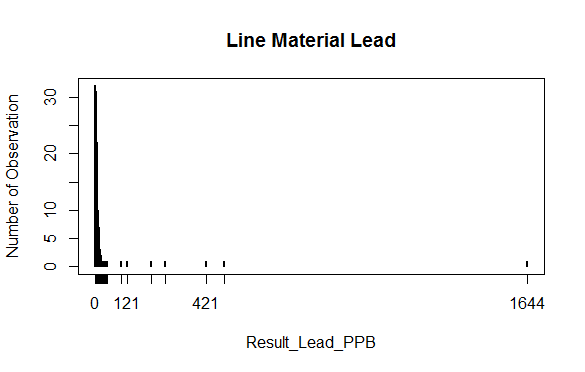
\includegraphics[width=7.0cm, height = 6cm]{Em_dis_Lead.png}}
  \centerline{(a)}
\end{minipage}
\hfill
\begin{minipage}{.48\linewidth}
  \centerline{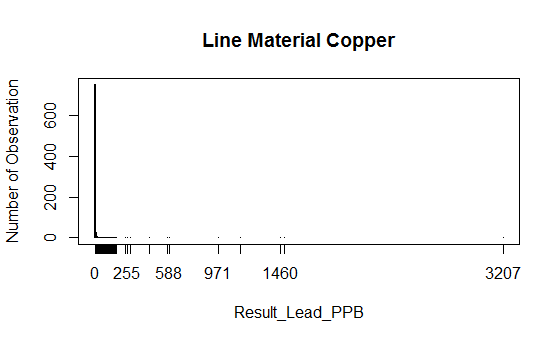
\includegraphics[width=7.0cm, height = 6cm]{Em_dis_Copper.png}}
  \centerline{(b)}
\end{minipage}
\vfill
\caption{Dot plot for lead level}
\label{fig:res}
\end{figure}
\end{center}

The generalized linear mixed effect model for the lead level in water has the following form:
\begin{center}
\large{$y_{ij} = \frac{exp(x_{ij}^T \beta + d_{ij}^{T}U_{i} + \epsilon_{ij})}{1 + exp(x_{ij}^T \beta + d_{ij}^{T}U_{i} + \epsilon_{ij})}$}
\end{center}
Here, $y_{ij}$ equals to 0 or 1, denoting whether the lead level would be greater than 15 PPB or not. $X_{ij}$ are the fixed treatments, which includes the treatments of service line material and zip codes. $U_{i}$ is the random vector, which has 0 mean and constant variance. $\beta$ is the coefficient vector of the random effect, and $d_{ij}$  is the design matrix. $\epsilon$ is the random error for each observation.  

Then, I used lme4 package in R to fit the model. The fitting outcome is shown in list 1
\lstinputlisting[float=h,frame=tb,caption=Summary of lead model,label=zebra]{Model_lead.txt}

In the estimation for the fixed part of the model, the intercept denotes the situation that using copper water pipe in zip code 48503. According to the p-value, it can say that in 48503, using lead pipe would contribute more to the probability of whether the lead level in the water is greater than 15 than using copper pipe. And if all using copper pipes, the probability for lead level higher than 15 PPB in 48505 and 48507 would be much smaller, since the estimation of these two coefficient are significant and are less than 0. And for random effect part, the estimation for variance component is about 3.85, which shows that the sample location do have some random effect for the observations.

Here, the estimate for Service line material lead denotes the difference of contribution when using lead pipes and using copper pipes. The 95\% confidence interval of the estimate is $[0.026, 1.202]$. So the coefficient would significantly larger than 0. Then it can show that using lead pipes would more possible to make the lead level in the water higher than 15 PPB. 

In further, I want to explore whether there are any interaction between the fixed treatments. So I refitted the model and include the interaction between the zip codes and the service line material. The outcome is shown below:
\lstinputlisting[float=h,frame=tb,caption=Summary of interaction model,label=zebra]{out_cross.txt}

\noindent The outcome above shows that the interaction between galvanized pipes and zip code 48505 have a significant estimate. This may indicate that they may have some relationship.

\noindent Then, I performed AIC comparision  to decide which model is better.
\lstinputlisting[float=h,frame=tb,caption=AIC Compare,label=zebra]{Likezip_lead.txt}

\noindent It shows that the model with interaction is better. So I choose this as my final model.

\section*{\sihao Model Diagnostic}
The Pearson residual plot is shown in Figure 2.
\begin{center}
\begin{figure}[h]
\begin{minipage}{0.48\linewidth}
  \centerline{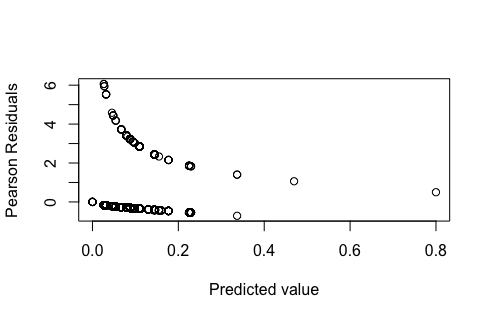
\includegraphics[width=7.0cm, height = 6cm]{log_res_lead.png}}
  \centerline{(a) Pearson Residual Plot}
\end{minipage}
\hfill
\begin{minipage}{.48\linewidth}
  \centerline{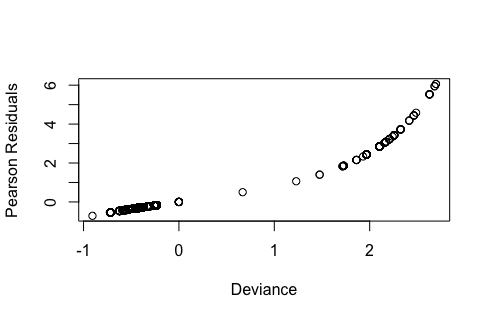
\includegraphics[width=7.0cm, height = 6cm]{Dev_res.png}}
  \centerline{(b)Deviance - Pearson Residuals}
\end{minipage}
\vfill
\caption{Residual plots}
\label{fig:res}
\end{figure}
\end{center}
The plot shows that most data points are distributed approximately beside the horizontal line $y = 0$. Several outliers have residuals greater than 3. Compared with the number of total observations, outliers are not so many. So the model is somehow appropriate. As for the deviance and Pearson residual plot, it shows that there are some outliers. It make sense because the original observations are mostly equal to 0. There distribution of them is not normal, so the model is not stable.

Then I applied a likelihood ratio test to see the significance of all the parameters. The hypothesis is in following way:
\begin{center}
$H_{0}: \beta_{1} = \beta_{2}=... \beta_{k} = 0, \quad H_{1}: \exists \beta_{i} \neq 0$
\end{center}
In R, I applied anova function to get the result of the likelihood ratio test. 
\lstinputlisting[float=h,frame=tb,caption=Likelihood ratio test for Lead Model,label=zebra]{liketest_lead.txt}

\noindent By doing the $\chi^2$ test, it shows that the full model is much better than the reduced model, in which there is no predictors. So in this way, I can significantly refuse the Null hypothesis and say that the model is significant.







\section*{\sihao Predictions}
For the application of model, I use a new data set which contains new observations made in April, 2016. I apply the model to the new data set and make predictions. The critical value is obtained by using bootstrap. I randomly sample the observations from the existing data set to fit the model and get predicted values of the probability that a high lead level situation would happen. Then, I choose the 0.95 quantile point to be the critical value of the prediction. If the predicted value is greater than the critical value, then I assume the high level of lead incidence would happen. For the new data set, the prediction accuracy is about 0.8. In figure 3, I use ROC curve to show the performance of the model in training set. 
\begin{center}
\begin{figure}[ht]
\quad  \quad \quad 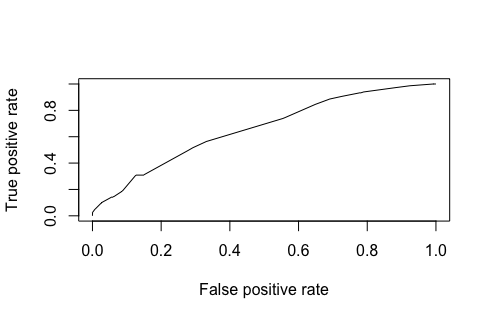
\includegraphics[width = 12cm, height = 8cm]{Roc_predict.png}
\vfill
\caption{ROC curve}
\label{fig:res}
\end{figure}
\end{center}
The figure shows that the performance of the model in prediction is not very good. But obviously, it is better than random guess. The ratio of true positive rate and false positive rate is approximate to 0.5, which indicates that when the model predict a response variable to 1, it is more likely to do a random guess. And it is appropriate to our data set, because among our data set, most response variables are equal to 0 in the original data set. So if a predicted value is 0, then it make less likely to make a mistake. So when doing predictions, we can set the critical value a little bit higher, so that we can avoid to predict the response equal to 1. In this way, we can minimize the error rate.

\section*{\sihao Conclusion}
From the surveys data, it can see that the lead and copper contamination in Flint water system is not so severe now, since many observations shows that there is no lead and copper in the water. But in some areas, extremely high lead contamination (lead level larger than 15 PPB) still exists, which shows that the water crisis does not disappear.

By using generalized linear fixed effect model, I found that the lead contamination do have been influenced by the material of water pipes, especially lead pipes. When using lead pipes, it is more likely to cause a extremely high lead contamination than using copper pipes. So if possible, changing lead pipes to copper pipes would help the reduce the probability of be affected by lead in the water. Further, in some areas like 48505 and 48507, the probability of highly contamination would be significantly reduced. It may indicate that in these areas, water quality is better.

Finally, when doing prediction, it is better to set the critical value a little bit higher. It is due to the large proportion of 0 existing in the data set. 
\end{document}





























